\documentclass[10pt]{article}
% Эта строка — комментарий, она не будет показана в выходном файле
\usepackage{ucs}
\usepackage[utf8x]{inputenc} % Включаем поддержку UTF8
\usepackage[russian]{babel}  % Включаем пакет для поддержки русского языка
\usepackage{amsmath}
\usepackage{amssymb}
\usepackage{mathtools}

\hoffset=0mm
\voffset=0mm
\textwidth=170mm        % ширина текста
\oddsidemargin=-0mm   % левое поле 25.4 - 5.4 = 20 мм
\textheight=240mm       % высота текста 297 (A4) - 40
\topmargin=-15.4mm      % верхнее поле (10мм)
\headheight=5mm      % место для колонтитула
\headsep=5mm          % отступ после колонтитула
\footskip=8mm         % отступ до нижнего колонтитула

\title{Лабораторная работа № 2.1:
    Определение $C_p/C_v$ по скорости звука в газе    
}
\date{\today}
\author{Миллер Сергей 494}

\begin{document}
    \maketitle
    \textbf{Цель работы:}1)  измерение частоты колебаний и длины волны при резонансе звуковых колебаний в газе, заполняющем трубу; 2) определение показателя адиабаты по скорости звука с помощью уравнения состояния идеального газа.

    \textbf{Теория.}

    \textbf{Звуковые волны.} 

    В простых гармонических звуковых волнах, распространяющихся вдоль оси $Ox$, изменение давления $\Delta P$ зависит от координаты $x$ и времени $t$ по закону

    \begin{equation}
        \Delta P(x,t) = P_0 cos(\omega t \pm kx).
    \end{equation}

    Два знака в аргументе косинуса соответствуют двум направлениям распространения волны. Между круговой частотой $\omega$, волновым числом $k$, длиной волны $\lambda$ и скоростью звука $v_\text{зв}$ выполняются соотношения

    \begin{equation}
        v_\text{зв} = \frac{\omega}{k} = \lambda f; \quad k = 2\pi; \quad \omega = 2\pi f;
    \end{equation}
    здесь $f$ — частота волны.
    Важной характеристикой звуковых волн является скорость их
    распространения. Она определяется инерционными и упругими свойствами среды. Скорость распространения продольных волн в безграничной однородной среде определяется выражением:
     
    \begin{equation}
        v_\text{зв} = \sqrt{\frac{dP}{d\rho}}.
    \end{equation}

    Давление $P$ зависит не только от плотности $\rho$, но и от темпе- ратуры $T$ . Поэтому нужно уточнить, в каком смысле понимается производная $\frac{dP}{d\rho}$.
    Колебания плотности и связанные с ними колебания темпера- туры в звуковой волне происходят настолько быстро, а теплопроводности газов настолько малы, что для таких процессов теплообменом можно пренебречь, так что процесс распространения звука можно считать \textit{адиабатическим}. Следовательно, производную $\frac{dP}{d\rho}$ необходимо рассчитывать для адиабатического процесса.


    \textbf{ Первое начало термодинамики.}

    Из закона сохранения энергии следует, что тепло $Q$, полученное термодинамической системой, расходуется на изменение её внутренней энергии $\Delta U$ и на совершение работы $A$ над внешними телами:
    \begin{equation}
        Q = \Delta U + A
    \end{equation}
    Для бесконечно малого процесса уравнение (4) принимает вид 
    \begin{equation}
        \delta Q = dU + \delta A
    \end{equation}

    Поскольку внутренняя энергия является функцией состояния системы, для её элементарного приращения использован знак полного дифференциала $dU$ , а приращения и тепла, и работы не являются полными дифференциалами, а $Q$ и $A$ — не функции состояния(
    Для интегрирования должен быть задан весь промежуточный процесс, поскольку результат будет зависеть от его вида, а не только от начального и конечного состояний).

    \textbf{ Работа газа.}

    Рассмотрим расширение газа в цилиндре, закрытом подвижным поршнем. На поршень действует сила $F$ , равная произведению давления газа $F$ на площадь поршня $S$. При смещении на малую величину $dx$ газ совершает работу
    \begin{equation}
        \delta A = F dx = P S dx = P dV.
    \end{equation}
    где $dV$  — малое изменение объёма газа.
    Значит полная работа при некотором процессе имеет вид:
    \begin{equation}
        A = \int P(V) dV
    \end{equation}
    А первое начало термодинамики для газов после использования формулы (6) будет иметь вид:
    \begin{equation}
        \delta Q = dU + P dV
    \end{equation}

    \textbf{Теплоемкость}
    Отношение количества тепла $\delta Q$, поглощённого $\nu$ молями газа при некотором процессе, который обозначим индексом $x$, к повышению его температуры на $dT$, делённое на число молей $\nu$, называется \textit{молярной теплоемкостью газа}:

    \begin{equation}
        C = \bigg(\frac{\delta Q}{dT}\bigg)_x / \nu
    \end{equation}

    Будем считать что $U = U(V,T)$ (так как система описывается тремя параметрами: $V,T,P$ но при этом есть уравнение Менделеева-Клапейрона: $P = P(V,T)$).
    Значит полный дифференциал для $U$ имеет следующий вид:

    \begin{equation}
        dU = \bigg(\frac{\delta U}{\delta T}\bigg)_V dT + \bigg(\frac{\delta U}{\delta V}\bigg)_T dV
    \end{equation}

    Подставим его в первое начало термодинамики:

    $  \delta Q = dU + \delta A =  \bigg(\frac{\delta U}{\delta T}\bigg)_V dT + \bigg(\frac{\delta U}{\delta V}\bigg)_T dV + PdV = \bigg(\frac{\delta U}{\delta T}\bigg)_V dT + \bigg[P + \bigg(\frac{\delta U}{\delta V}\bigg)_T \bigg] dV $

    Разделив все на $dT$ найдем теплоемкость $C_x$ в процессе x:

    \begin{equation}
        C_x = C_v + \bigg[P + \bigg(\frac{\delta U}{\delta V}\bigg)_T \bigg] \bigg(\frac{\delta V}{\delta T}\bigg)_x
    \end{equation}

    Здесь производная $\bigg(\frac{\delta V}{\delta T}\bigg)_x$ вычисляется с учётом процесса $x$, при котором происходит подвод тепла, например, при постоянном объёме $(𝑥 = 𝑉 )$, при постоянном давлении $(𝑥 = 𝑃 )$ или другом условии. Величина $C_v = \bigg(\frac{\delta U}{\delta T}\bigg)_V$ в формуле (11) является теплоёмкостью при постоянном объёме(Дейсвительно, это определение совпадает с определением теплоемкости, так как в процессе $V = const$ выполняется $\delta A = 0$ а значит $\detta U = dQ$).

    \textbf{Теплоёмкость идеального газа.}
    В модели идеального газа внутренняя энергия определяется только кинетической энергией движения молекул, следовательно, внутренняя энергия идеального газа не зависит от объёма: $\bigg(\frac{\delta U}{\delta V}\bigg)_T = 0$.

    Тогда формула (11) станет более простой:

    \begin{equation}
        C_x = C_v + P \bigg(\frac{\delta V}{\delta T}\bigg)_x
    \end{equation}

    Используя уравнение Менделеева-Клапейрона ($PV = \nu RT$),
    для $C_p$ (то есть процесса $x = P$ с постоянным давлением) получим:

    \begin{equation}
        C_p - C_v = R
    \end{equation}
    где $C_p, C_v$ - \textit{молярные} теплоемкости при постоянных давлении и объеме соответсвенно.

    Отношение этих теплоемкостей называется показателем адиабаты:

    \begin{equation}
        \gamma = \frac{C_p}{C_v}
    \end{equation}

    В нешироком диапазоне температур $C_v$ можно считать постоянной, что соответствует пропорциональности внутренней энергии газа его температуре:

    \begin{equation}
        U = \nu \int C_v dT = \nu C_v T
    \end{equation}

    Энергия, переданная молекуле, распределяется между различными формами её движения: поступательным, вращательным и колебательным. В статистической физике доказывается теорема о равномерном распределении энергии между степенями свободы молекулы, согласно которой на каждую степень свободы приходится в среднем энергия, равная $\frac{RT}{2 N_A}$

    При $i$ степенях свободы, внутренняя энергия $U$ одного моля такого газа и величина $C_v$ равны соответственно

    \begin{equation}
        U = \frac{i}{2}RT; \quad C_v = \frac{iR}{2}; 
    \end{equation}

    где $R = 8,31 \text{Дж}/\text{(моль · К)}$ — универсальная газовая постоянная, $N_A = 6,02 · 1023 \text{моль}^{−1}$ — количество молекул в моле вещества (число Авогадро).
    В рассматриваемом приближении для показателя адиабаты в соответствии с (13) и (14) получим

    \begin{equation}
        \gamma = \frac{i+2}{i}
    \end{equation}

    \textbf{Адиабатический процесс.}

    Квазистатический процесс, происходящий без теплообмена с окружающей средой, называется адиабатическим.
    Из первого начала термодинамики (6) при $\delta Q = 0$ для $\nu$ молей идеального газа, у которого $dU = \nu C_v dT$, получим:

    \begin{equation}
        \nu C_v dt + P dV = 0,
    \end{equation}

    А так как $PV = \nu RT$, получаем: 

    \begin{equation}
        C_v \frac{dT}{T} + R \frac{dV}{V} = 0
    \end{equation}

    Далее интегрируя и вновь используя уравнение состояния, получим:

    \begin{equation}
        PV^{\gamma} = const
        \text{  (адиабата Пуассона)}
    \end{equation}

    \textbf{Скорость звука}

    Распространение звуковой волны в газе проис- ходит адиабатически. Сжатия и разрежения в газе сменяют друг друга настолько быстро, что теплообмен между слоями газа, имеющими разные температуры, не успевает произойти. Используя полученное уравнение адиабаты идеального газа, найдём скорость звука по общей формуле (3).

    Заменим в уравнении Пуассона $PV^{\gamma} = const$ объём на плот- ность $\rho = \frac{m}{V}$ , после чего получим $P = const \rho^{\gamma} $. Тогда после логарифмирования и дифференцирования этого выражения имеем:

    \begin{equation}
        \frac{dP}{P} = \gamma \frac {d\rho}{\rho}, \quad \text{или} \quad \bigg(\frac{dP}{d\rho}\bigg)_\text{адиаб} = \gamma \frac{P}{\rho},
    \end{equation}

    тогда для скорости звука получаем:

    \begin{equation}
        v_\text{зв}^2 = \bigg(\frac{dP}{d\rho}\bigg)_\text{адиаб} = \gamma \frac{P}{\rho} = \gamma \frac{RT}{\mu},
    \end{equation}
    где $\mu$ - молярная масса газа.

    Преобразуя, получим:

    \begin{equation}
        \gamma = \frac{\mu}{RT}v_\text{зв}^2
    \end{equation}

    Таким образом, для определения показателя адиабаты достаточно измерить температуру газа и скорость распространения звука (молярная масса газа предполагается известной).

    \textbf{Идея эксперимента}

    Звуковые колебания в трубе являются наложением всех отражённых волн и, вообще говоря, очень сложны. Картина упрощается, если длина трубы $𝐿$ равна целому числу полуволн, то есть когда выполняется условие
    \begin{equation}
        L = n\frac{\lambda}{2}
    \end{equation}
    где $n$ — любое целое число. Совпадающие по фазе волны, бегущие в противо- положных направлениях, складываясь, усиливают друг друга, и образуется стоячая звуковая волна:
    Δ𝑃 (𝑥,𝑡) = 2𝑃0 cos(𝜔𝑡) sin(𝑘𝑥).
    Амплитуда звуковых колебаний при этом резко возрастает - наступает резонанс.

    При неизменной частоте 𝑓 звукового генератора (а следовательно, и неизменной длине звуковой волны $\lambda$) можно изменять длину трубы 𝐿. Для этого применяется раздвижная труба. Длина раздвижной трубы постепенно увеличивается, и наблюдается ряд последовательных резонансов. Возникновение резонанса легко наблюдать на осциллографе по резкому увеличению амплитуды колебаний. Для последовательных резонансов имеем

    \begin{equation}
        L_n = n\frac{\lambda}{2}, L_{n+1} = (n+1)\frac{\lambda}{2}, \dots L_{n+k} = n\frac{\lambda}{2} + k\frac{\lambda}{2}
    \end{equation}
    
    т. е. $\lambda/2$ равно угловому коэффициенту графика, изобража- ющего зависимость длины трубы $L$ от номера резонанса $k$. Скорость звука находится по формуле (2).

    \textbf{В работе испольуются:} звуковой генератор (ЗГ); электронный осциллограф (ЭО); микрофон; раздвижная труба; термометр.

    \begin{center} 
    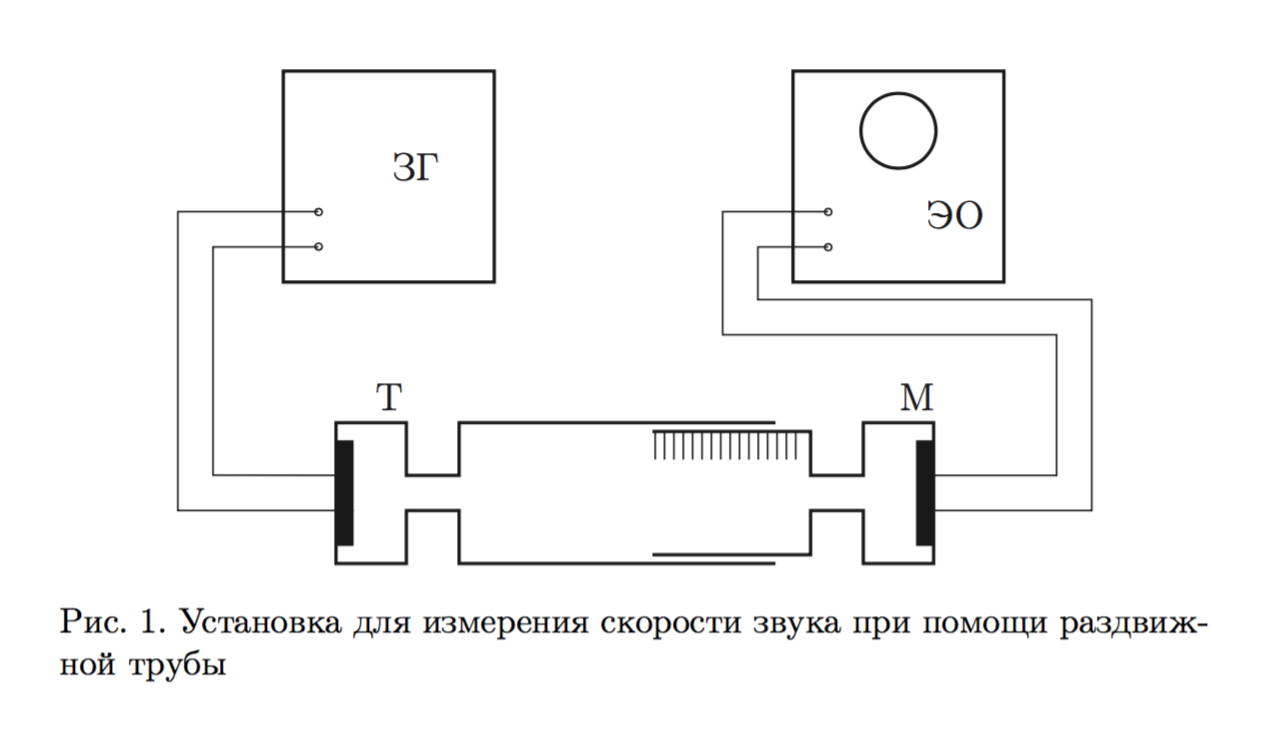
\includegraphics[width=3.5in]{stand.png}
    \end{center}

    \textbf{Ход работы:}

    \begin{enumerate}
    \item 
         Будем медленно удлинять трубу при постоянной частоте и измерять смещение трубы от начального состояния при последовательных резонансах.
    Так как ожидаемая зависимость длины трубы от номера резонанса $\Delta(n)$ линейная, то для случаев $n > 2$ (иначе оценим непосредственно) построим аппроксимирующие по методу наименьших квадратов прямые вида $\Delta = kn + b$ для каждой измеряемой частоты, а также произведем оценку ошибки(для углового коэффицента $k$):

    \begin{equation}
        \hat{k} = \frac{\overline{xy} - \bar{x}\bar{y}}{\overline{x^2} - \bar{x}^2} ;\quad \hat{\sigma}_k = \frac{2}{\sqrt{n}}\sqrt{\frac{\overline{y^2} - \bar{y}^2}{\overline{x^2} - \bar{x}^2} - \hat{k}^2}
    \end{equation}

    Здесь в качестве погрешности для полученной оценки $\hat{k}$  взяли удвоенное стандартное отклонение, в пределах которого в среднем лежит $98\%$ результатов.

    После этого найдем скорость звука: $\hat{v}_\text{зв} = \hat{\lambda} f = 2 \hat{k} f$

    Тогда получим искомое значение показателя адиабаты: $\hat{\gamma} = \frac{4\mu \hat{k}^2 f^2}{RT}$ 

    А погрешности $\sigma_\gamma, \sigma_{v_\text{зв.}}$ определим из формулы для погрешности функции многих переменных:

    \begin{equation}
        \bigg(\frac{\sigma_\gamma}{\gamma}\bigg) ^ 2 =    2^2 \bigg(\frac{\hat{\sigma}_k}{\hat{k}}\bigg) ^ 2 + 2^2 \bigg(\frac{\sigma_f}{f}\bigg) ^ 2 + \bigg(\frac{\sigma_T}{T}\bigg) ^ 2 
    \end{equation}
    \begin{equation}
        \bigg(\frac{\sigma_{v_\text{зв.}}}{v_\text{зв.}}\bigg) ^ 2 =    \bigg(\frac{\hat{\sigma}_k}{\hat{k}}\bigg) ^ 2 + \bigg(\frac{\sigma_f}{f}\bigg) ^ 2
    \end{equation}


    При измерениях:

        $\sigma_T = 0.1 K$ (половина цены деления термометра), $ \frac{\sigma_f}{f} = 0.01 $ (шкала ЗГ показывала 2 значащие цифры после запятой в измеряемом диапазоне)
        Поскольку измерения при движении трубы в обе стороны давали результаты отличающиеся не более чем на 1 мм то для расчетов использовались усредненные измерения каждого резонанса в обе стороны. 
  
    \begin{itemize}
        \item $f = 1.13$ KГц,$ \quad T = 21.6^o C$

        \begin{center}
                    \begin{tabular}{|c|c|c|}
                            \hline 
                                $n$ & 1 & 2 \\
                            \hline
                                $\Delta_n$ [мм]& 75&220\\
                            \hline
                    \end{tabular}
        \end{center}

        (т. к. $n = 2$ в рассчете $\hat{\sigma}_k$ использована удвоенная приборная погрешность для линейки)
        \begin{equation}
            \hat{k} = 145.0 , \quad \hat{\sigma}_k = 5.8, \quad v_\text{зв.} = 327.7, \quad \sigma_{v_\text{зв.}} = 9.6 , \quad \varepsilon_{v_\text{зв.}}  \approx 4\% \quad \gamma = 1.27, \quad \sigma_\gamma = 0.13, \quad \varepsilon_\gamma \approx 10\%
        \end{equation}

        \begin{center} 
            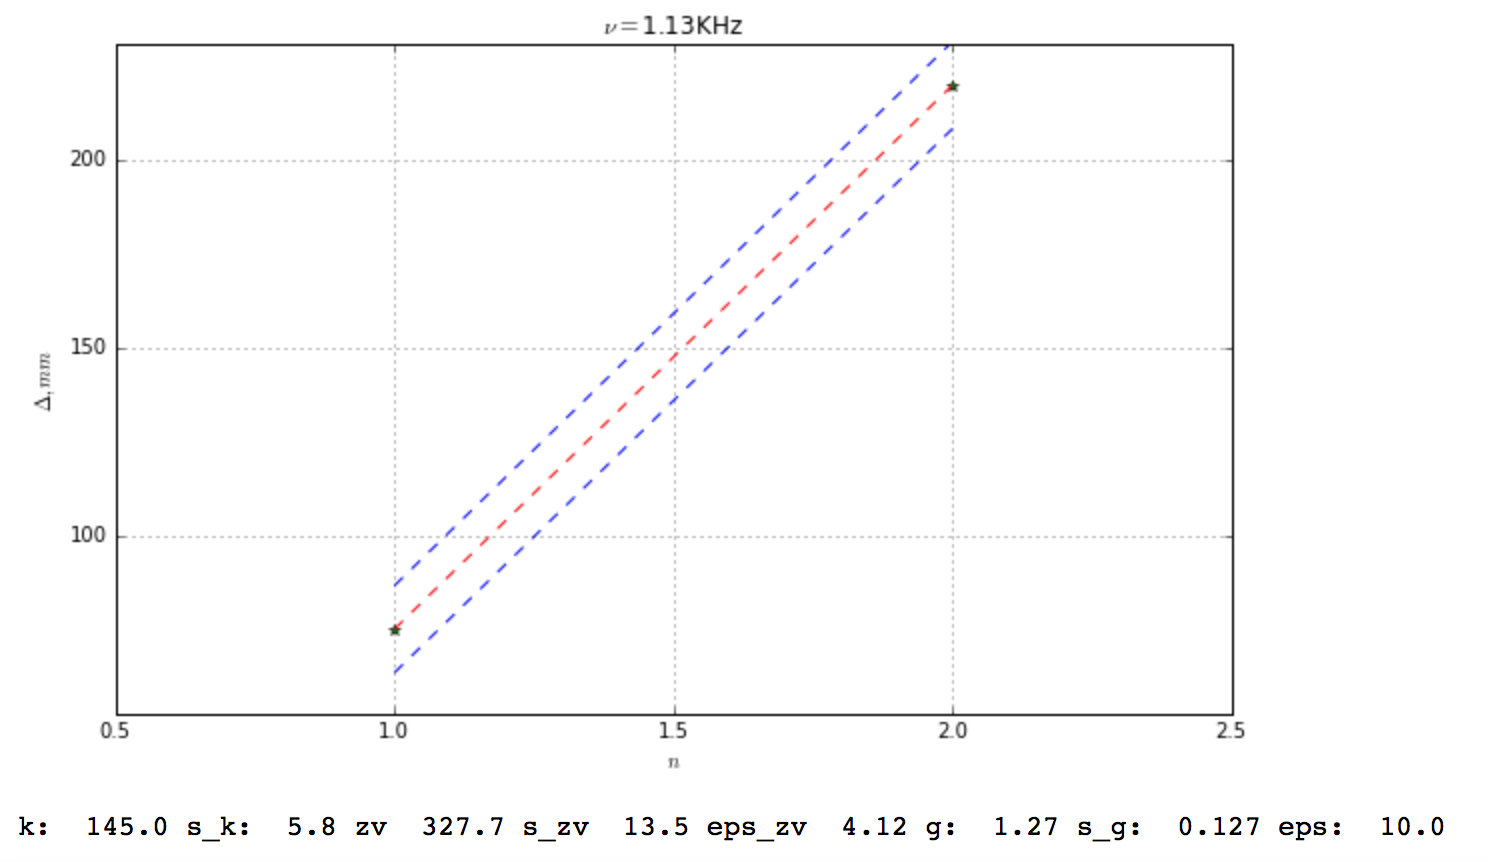
\includegraphics[width=5in]{1ex.png}
        \end{center}

        \item $f = 2.64$ KГц,$ \quad T = 21.6^o C$

        \begin{center}
                    \begin{tabular}{|c|c|c|c|c|c|}
                            \hline 
                                $n$ & 1 & 2 & 3 & 4  \\
                            \hline
                                $\Delta_n$ [мм]& 20&83&150&215\\
                            \hline
                    \end{tabular}
        \end{center}

        \begin{equation}
            \hat{k} = 65.2 ,\quad \hat{\sigma}_k = 0.8, \quad v_\text{зв.} = 344.3, \quad \sigma_{v_\text{зв.}} = 5.2 \quad \varepsilon_{v_\text{зв.}} \approx 1.5\% \quad \gamma = 1.41, \quad \sigma_\gamma = 0.09, \quad \varepsilon_\gamma \approx 6.5\%
        \end{equation}

        \begin{center} 
            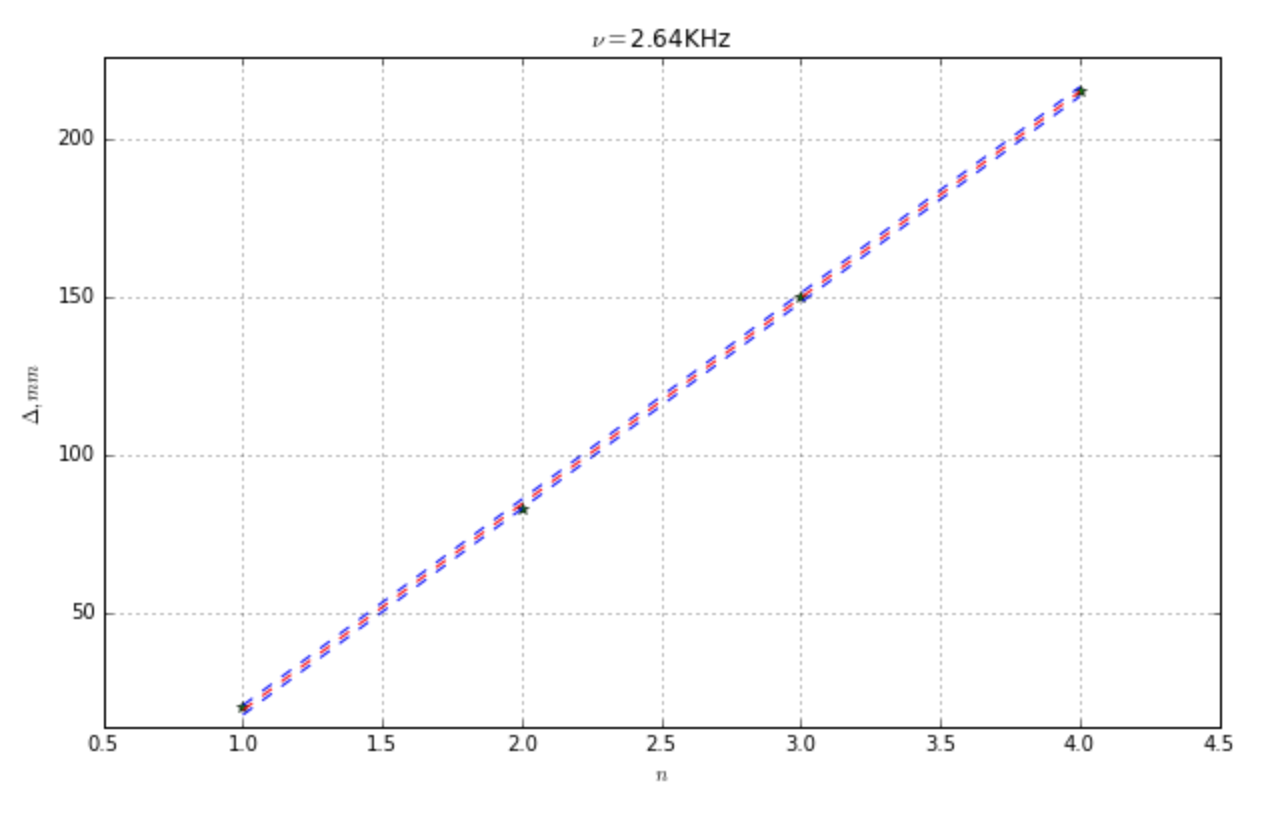
\includegraphics[width=5in]{2ex.png}
        \end{center}


        \item $f = 3.40$ KГц,$ \quad T = 21.2^o C$

        \begin{center}
                    \begin{tabular}{|c|c|c|c|c|c|c|}
                            \hline 
                                $n$ & 1 & 2 & 3 & 4 & 5 \\
                            \hline
                                $\Delta_n$ [мм]& 18&68&120&170&220\\
                            \hline
                    \end{tabular}
        \end{center}

        \begin{equation}
            \hat{k} = 50.6 ,\quad \hat{\sigma}_k = 0.3, \quad v_\text{зв.} = 344.1, \quad \sigma_{v_\text{зв.}} = 4.0 \quad \varepsilon_{v_\text{зв.}} \approx 1.2\% \quad \gamma = 1.41, \quad \sigma_\gamma = 0.09, \quad \varepsilon_\gamma \approx 6.1\%
        \end{equation}

        \begin{center} 
            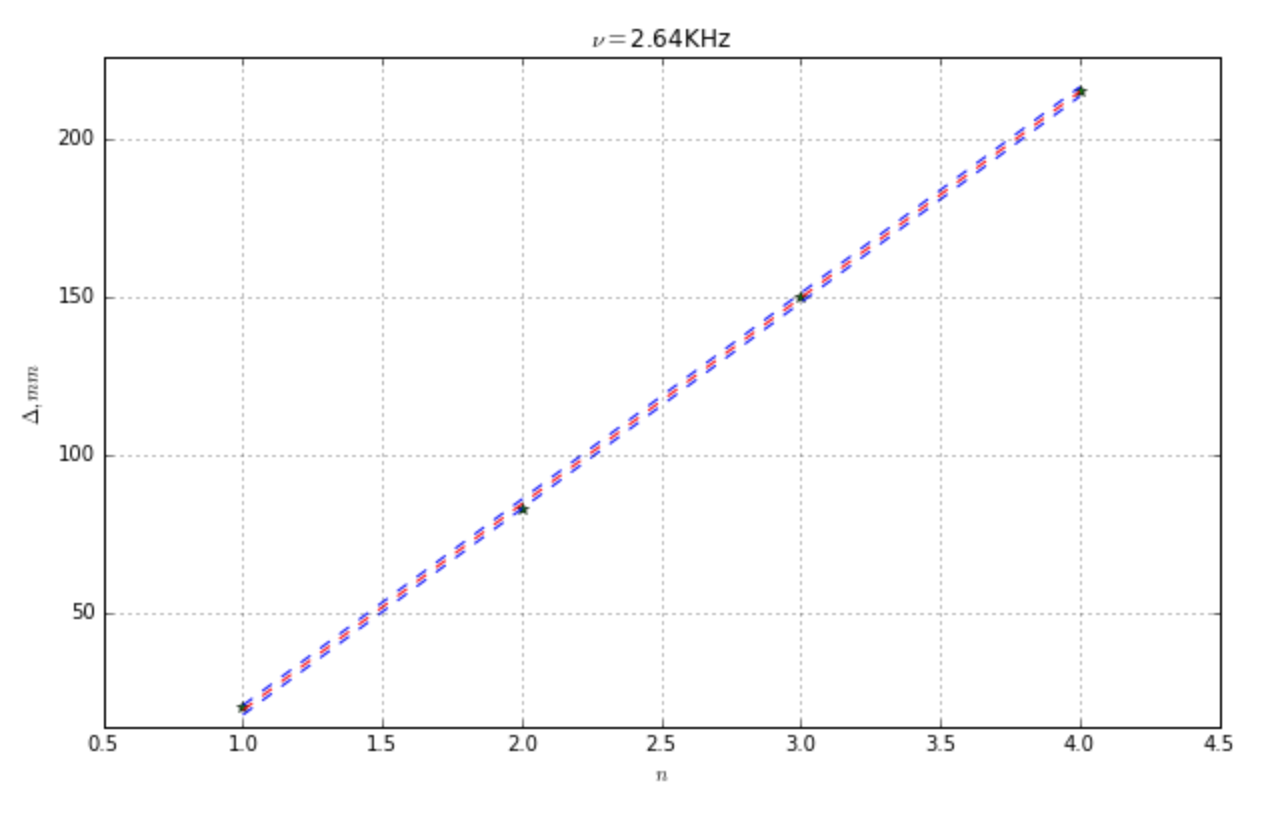
\includegraphics[width=5in]{2ex.png}
        \end{center}

        \item $f = 4.29$ KГц,$ \quad T = 21.2^o C$

        \begin{center}
                    \begin{tabular}{|c|c|c|c|c|c|c|c|}
                            \hline 
                                $n$ & 1 & 2 & 3 & 4 & 5 & 6 \\
                            \hline
                                $\Delta_n$ [мм]& 25&67&106&147&187&227\\
                            \hline
                    \end{tabular}
        \end{center}

        \begin{equation}
            \hat{k} = 40.3 ,\quad \hat{\sigma}_k = 0.3, \quad v_\text{зв.} = 345.9, \quad \sigma_{v_\text{зв.}} = 4.1 \quad \varepsilon_{v_\text{зв.}} \approx 1.2\% \quad \gamma = 1.42, \quad \sigma_\gamma = 0.09, \quad \varepsilon_\gamma \approx 6.1\%
        \end{equation}

        \begin{center} 
            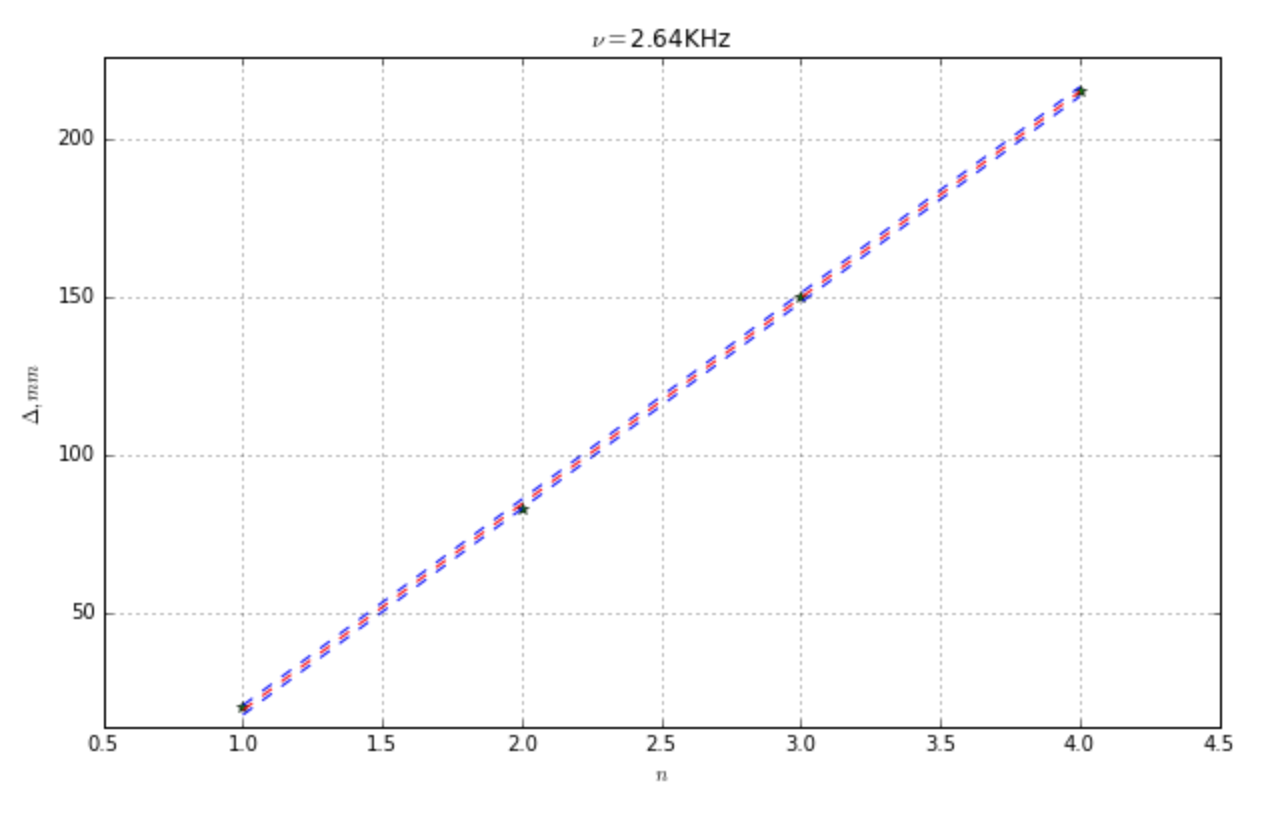
\includegraphics[width=5in]{2ex.png}
        \end{center}

        \item $f = 5.11$ KГц,,$ \quad T = 21.2^o C$

        \begin{center}
                    \begin{tabular}{|c|c|c|c|c|c|c|c|c|c|}
                            \hline 
                                $n$ & 1 & 2 & 3 & 4 & 5 & 6 & 7 \\
                            \hline
                                $\Delta_n$ [мм]& 10&44&77&112&145&180&212\\
                            \hline
                    \end{tabular}
        \end{center}

        \begin{equation}
            \hat{k} = 33.8 ,\quad \hat{\sigma}_k = 0.2, \quad v_\text{зв.} = 345.3, \quad \sigma_{v_\text{зв.}} = 4.1 \quad \varepsilon_{v_\text{зв.}} \approx 1.2\% \quad \gamma = 1.42, \quad \sigma_\gamma = 0.09, \quad \varepsilon_\gamma \approx 6.1\%
        \end{equation}

        \begin{center} 
            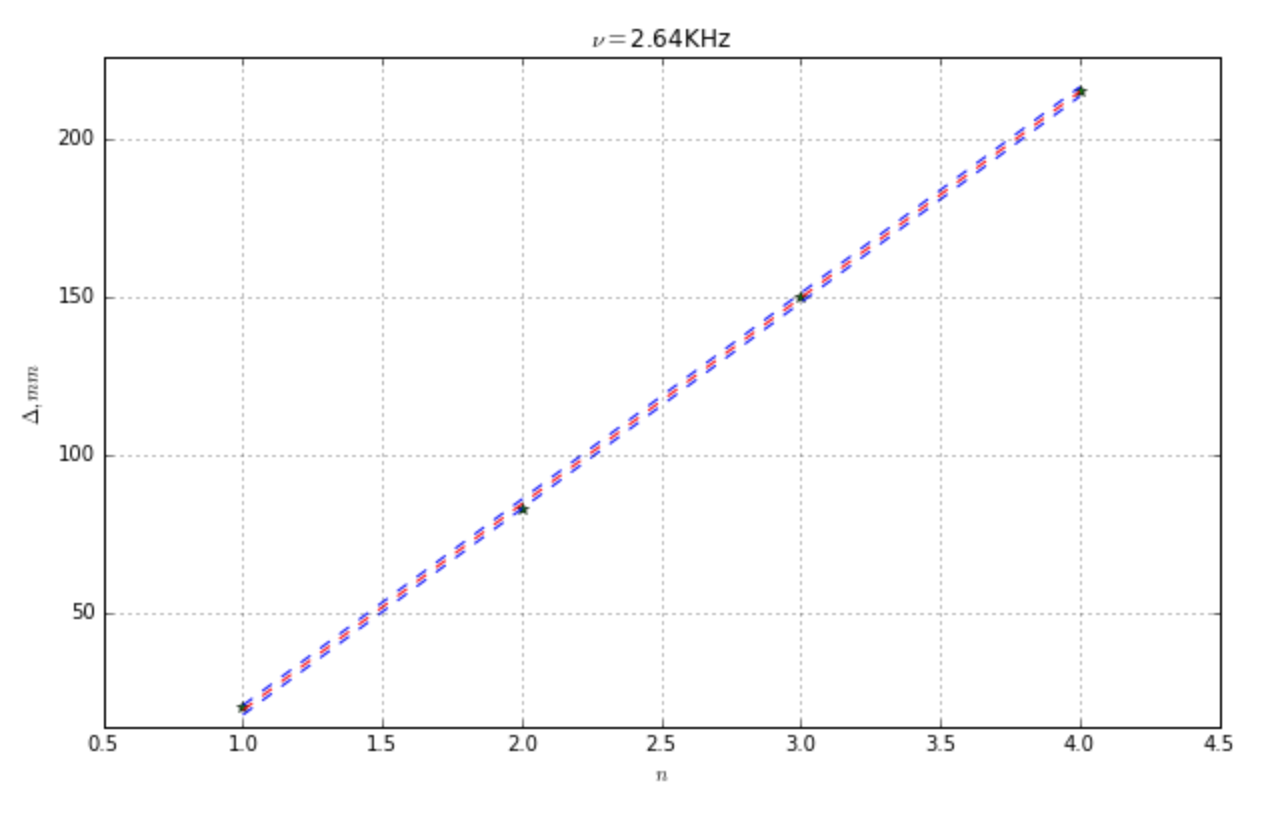
\includegraphics[width=5in]{2ex.png}
        \end{center}

    \end{itemize}

    \end{enumerate}

    Видно, что серия экспериментов при частоте $f = 1.13\text{КГц}$ имеет очень большую погрешность и малую достоверность, поэтому при расчете среднего значения $\gamma$ эту серию экспериментов лучше не учитывать.

    Усредняя результат по остальным независимым сериям, получим:

    \begin{equation}
        v_\text{зв.} = 344.9 \quad \sigma_{v_\text{зв.}} = \sqrt{\frac{\sigma_{{v_\text{зв.}}_2}^2 + \dots \sigma_{{v_\text{зв.}}_5}^2}{4}} = 4.4 
    \end{equation}
    \begin{equation}
        \gamma_\text{ex.} = 1.41 \quad \sigma_\gamma = \sqrt{\frac{\sigma_{\gamma_2}^2 + \dots \sigma_{\gamma_5}^2}{4}} = 0.09 
    \end{equation}

    в итоге получим эксперементальные значения:

    \begin{equation}
        v_\text{зв.ex.} = 344.9 \pm 4.4 \text{м/с}, \quad \gamma_{ex.} = 1.41 \pm 0.09
    \end{equation}

    используя физические таблицы для скорости звука в воздухе при $T ~ 20^o C$ и
    учитывая что воздух состоит примерно на 98\% из двухатомного газа($i = 5$ степеней свободы) то в теории для него примерно верно:

    \begin{equation}
         v_\text{зв.th.} \approx 343.1 \text{м/с} \quad \gamma_\text{th.} \approx \frac{i+2}{i} = 1.4
    \end{equation}

    Полученные значения с учетом погрешности позволяют говорить о применимости модели идеального газа для физических рассчетов в небольшом диапазоне температур.

\end{document}
